\hypertarget{metodología}{%
  \section{Metodología}\label{Metodología}}

\subsection{Enfoque de la investigación}

En esta investigación se empleará un enfoque cuantitativo, con el objetivo de analizar de manera objetiva y cuantificable
la relación entre la resolución de la guía de programación y el éxito académico en el curso de Introducción a la
Programación de la Universidad Andrés Bello.

\subsection{Diseño de investigación}

En este estudio, se empleará la metodología KDD (Knowledge Discovery in Databases, descubrimiento de conocimiento en bases de datos) para llevar a cabo el análisis de los datos. El proceso de KDD consta de varias etapas fundamentales que nos permitirán obtener conocimientos relevantes a partir de los datos recopilados. Estas etapas incluyen:

\textbf{Selección de datos}: En esta etapa, se identificarán y seleccionarán los datos relevantes para el estudio. En nuestro caso, utilizaremos el conjunto de datos "dataset a 2021" que contiene información sobre los resultados de la guía de programación y el rendimiento en la primera evaluación del curso de Introducción a la Programación en la Universidad Andrés Bello en el año 2021.

\textbf{Preparación de datos}: En esta etapa, se realizarán las transformaciones necesarias en los datos seleccionados para garantizar su calidad y adecuación al análisis. Esto puede incluir la limpieza de datos, la eliminación de valores atípicos o faltantes, y la normalización de variables, entre otros procesos.

\textbf{Minería de datos}: En esta etapa, se aplicarán técnicas de minería de datos para descubrir patrones, relaciones y tendencias ocultas en los datos. Utilizaremos técnicas estadísticas y algoritmos de aprendizaje automático para explorar la relación entre la resolución de la guía de programación, el éxito académico y el programa de estudio de los estudiantes.

\textbf{Evaluación de resultados}: En esta etapa, se evaluarán los resultados obtenidos a través de la minería de datos. Se analizarán los patrones identificados, se medirá su significancia estadística y se evaluará su relevancia para los objetivos de la investigación.

\textbf{Interpretación de hallazgos}: Finalmente, en esta etapa, se interpretarán los hallazgos obtenidos a partir del análisis de los datos. Se examinarán los resultados en el contexto de la pregunta de investigación planteada y se realizarán inferencias y conclusiones basadas en los patrones y relaciones descubiertos.

\begin{figure}[ht]
  \centering
  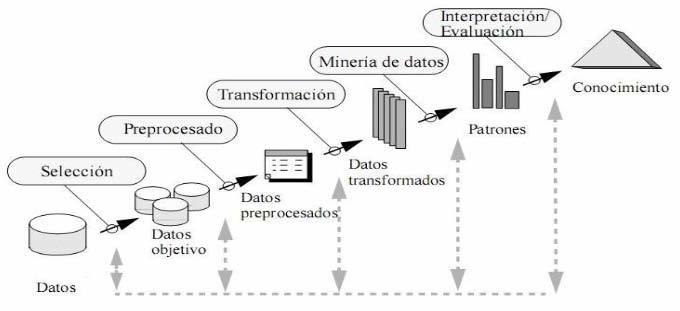
\includegraphics[width=4.06111in,height=2.68611in]{img/KDD.png}
  \caption{Flujo gráfico KDD}
  \label{fig:flujo_kdd}
\end{figure}

Al seguir la metodología KDD, nos aseguraremos de seguir un enfoque sistemático y riguroso para el análisis de los datos recopilados, lo que nos permitirá obtener conocimientos significativos y relevantes relacionados con la resolución de la guía de programación, el éxito académico y la deserción estudiantil en el curso de Introducción a la Programación en la Universidad Andrés Bello.


\subsection{Descripción de la base de datos}

El conjunto de datos utilizado en esta investigación se compone del registro de los estudiantes que tomaron el curso de
Introducción a la Programación en el año 2021 en la Universidad Andrés Bello. Estos datos incluyen información relacionada con la
resolución de la guía de apoyo para la primera evaluación.

La base de datos cuenta con un total de 839 registros y se compone de 75 columnas. Para el análisis,
se han seleccionado las siguientes columnas relevantes:

\begin{table}[htbp]
  \centering
  \caption{Descripción de variables}
  \begin{tabular}{|l|p{0.6\linewidth}|}
    \hline
    \textbf{Variable} & \textbf{Descripción}                                                                                                                                                               \\
    \hline
    sol1              & Representa la calificación obtenida en la primera evaluación, con un valor binario donde 1 indica una respuesta correcta a la pregunta, mientras que el valor predeterminado es 0. \\
    \hline
    exitosos          & Representa la cantidad de preguntas respondidas correctamente en la guía.                                                                                                          \\
    \hline
    fallidos          & Representa la cantidad de preguntas respondidas incorrectamente en la guía.                                                                                                        \\
    \hline
    envíos            & Representa la suma de respuestas exitosas y fallidas.                                                                                                                              \\
    \hline
    programa          & Representa al programa de estudio.                                                                                                                                                 \\
    \hline
  \end{tabular}
  \label{tab:variables}
\end{table}

Estas columnas son relevantes para nuestro análisis, ya que nos permitirán examinar la relación entre la resolución de la guía de programación,
el éxito académico en la primera evaluación y el programa de estudio al que pertenecen los estudiantes.


\subsection{Recopilación de datos}

Para llevar a cabo este estudio, se cuenta con el conjunto de datos denominado "dataset a 2021", que contiene la información necesaria sobre los
resultados de la guía de programación y el rendimiento en la primera evaluación del curso de Introducción a la Programación en el año 2021.


\subsection{Análisis de datos}

Una vez recopilados los datos, se realizará un análisis descriptivo para examinar la distribución de los resultados en la guía de programación y
la primera evaluación. Además, se llevará a cabo un análisis de correlación entre las variables mencionadas anteriormente para identificar posibles
relaciones y patrones significativos.
